\section{事例选择条件}
\label{sec:selection}
在物理分析过程中,经常利用探测器记录的末态粒子的相关信息,通过刻度和重建计算出带电径迹和中性径迹的径迹参数,并鉴别带电径迹的粒子类型,然后利用这些末态径迹重建出衰变过程中产生的各种中间共振态($\Ks,\pizero,\Lambda,\Sigma^0$和$\Sigma^+$)。
本节将详细的介绍好的带电粒子和好的中性粒子的鉴别方法,以及各种中间共振态的选择,见图~\ref{fig:intermediate}。
%%%%%%%%%%%%%%%%%%%%%%%%%%%%
\begin{figure*}[hp]
\centering
\subfigure[数据中$\pi^{0}$ 不变质量分布。]
{
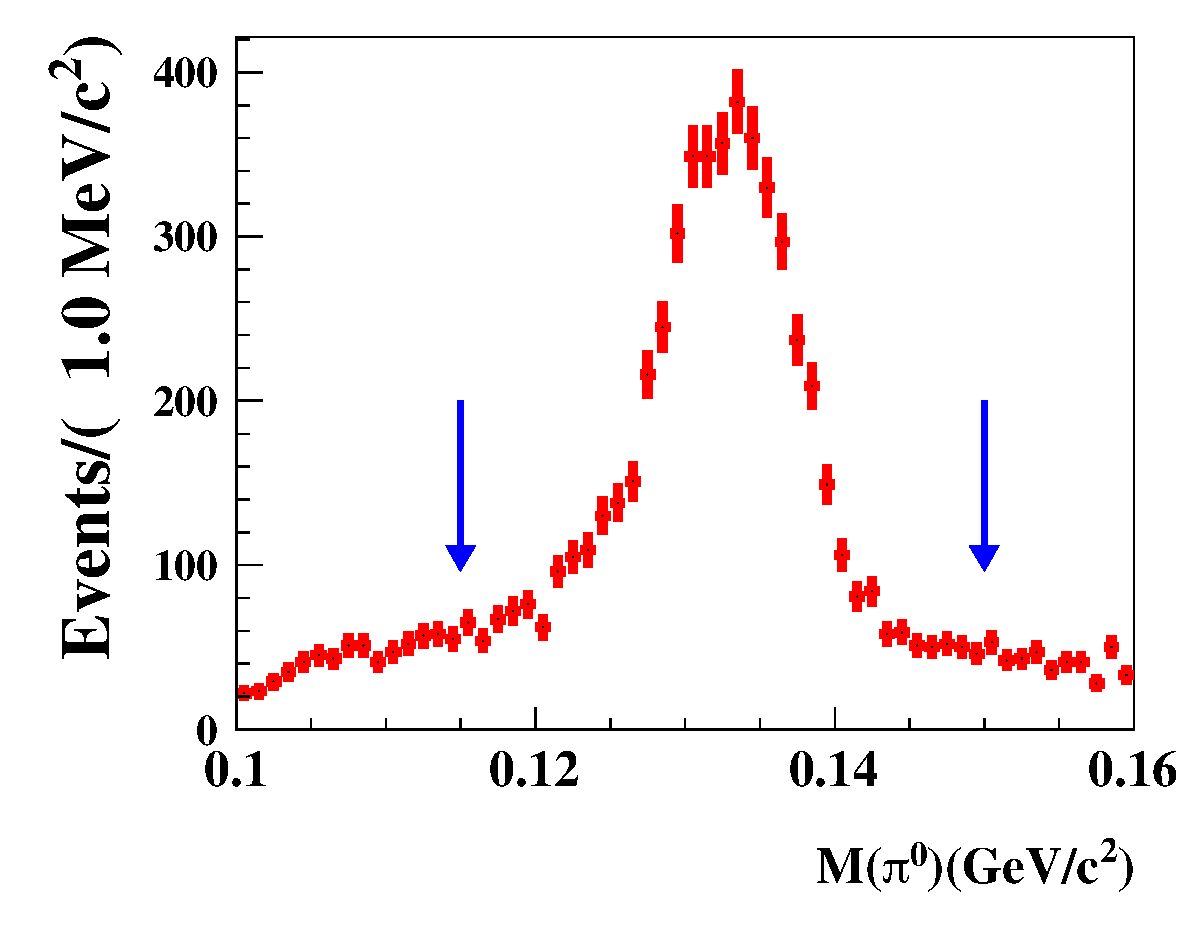
\includegraphics[width=0.45\textwidth]{chap2_m_pi0}
\label{fig:pi0mass}
}
\hspace{10pt}
\subfigure[数据中$K_{S}^{0}$ 不变质量分布。]
{
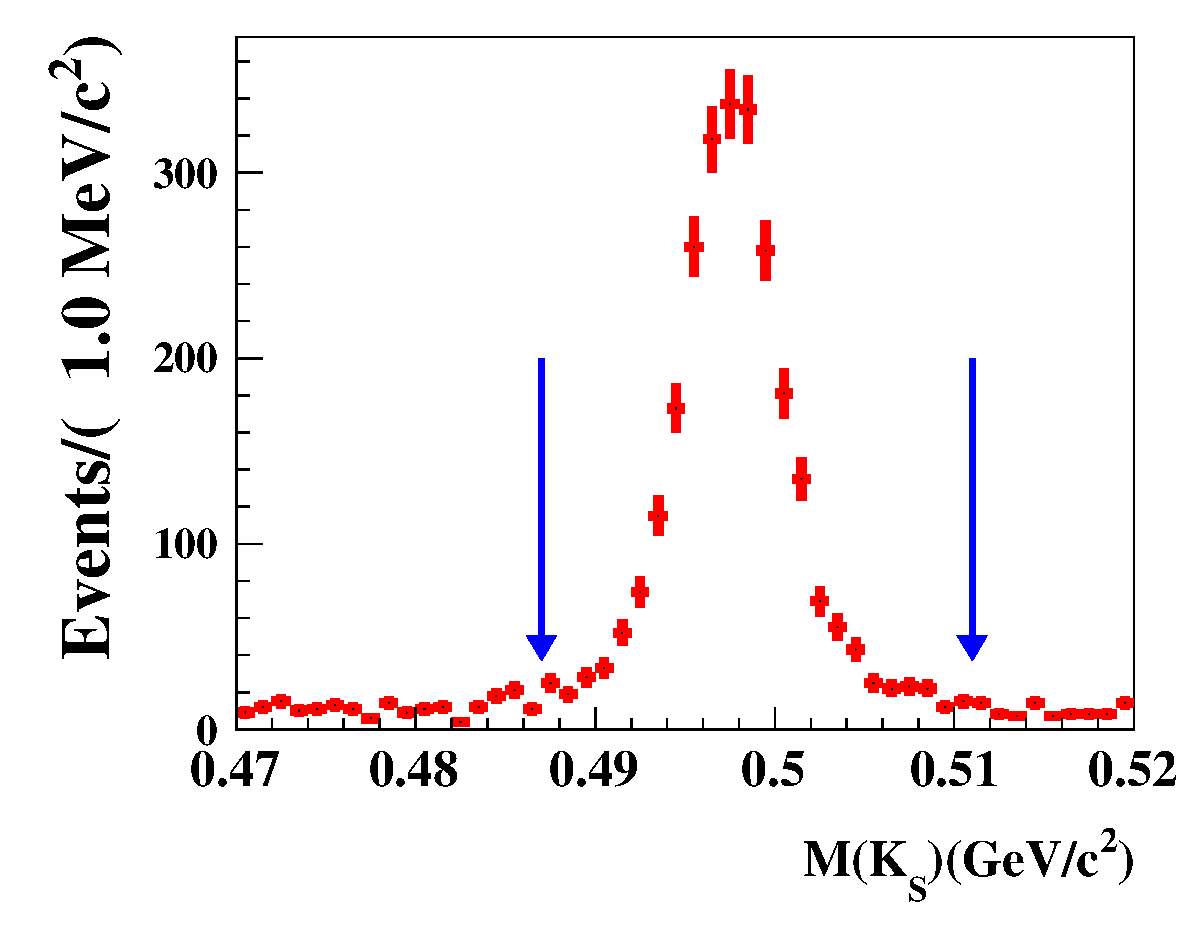
\includegraphics[width=0.45\textwidth]{chap2_m_Ks}
\label{fig:Ksmass}
}
\subfigure[数据中$\Lambda$ 不变质量分布。]
{
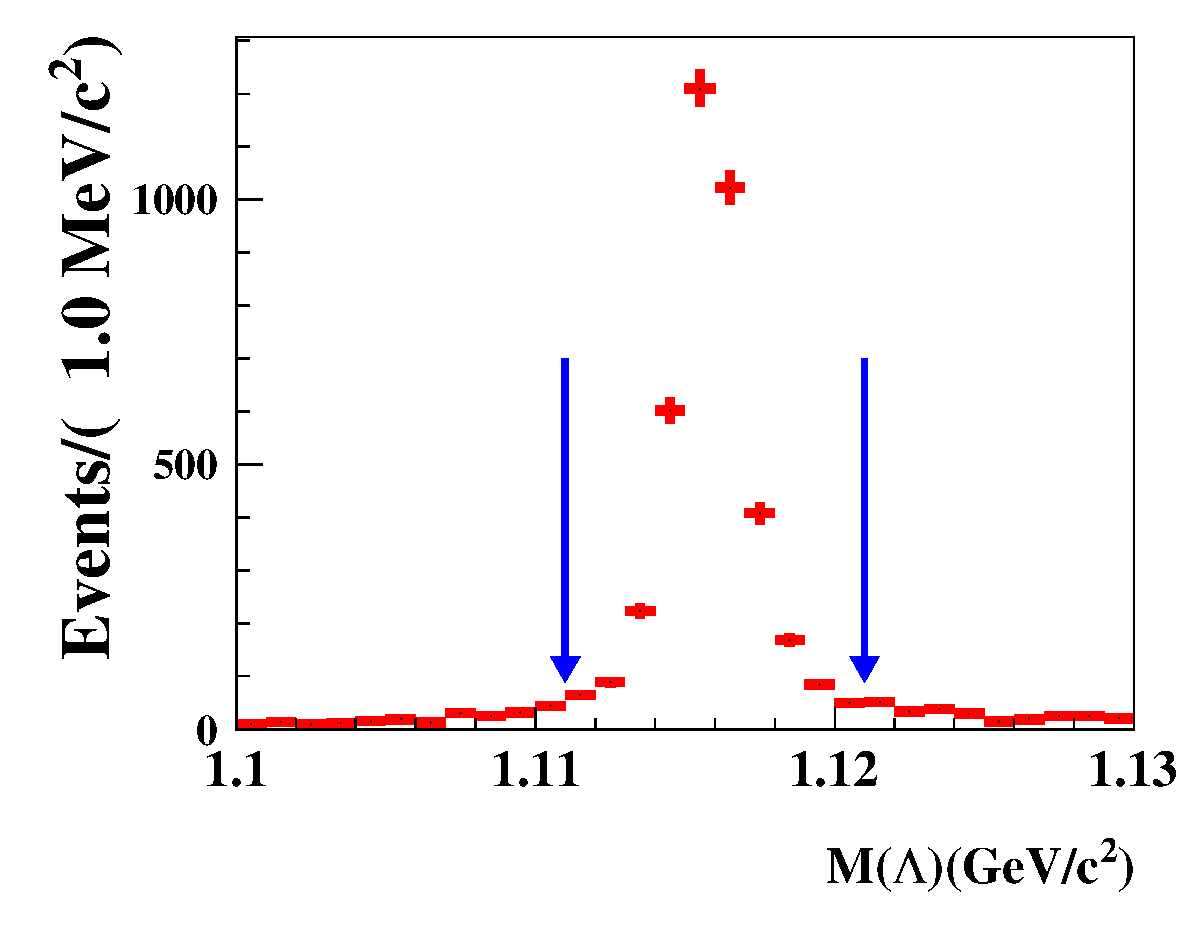
\includegraphics[width=0.45\textwidth]{chap2_m_lmd}
\label{fig:lmdmass}
}
\subfigure[数据中$\Sigmazero$ 不变质量分布。]
{
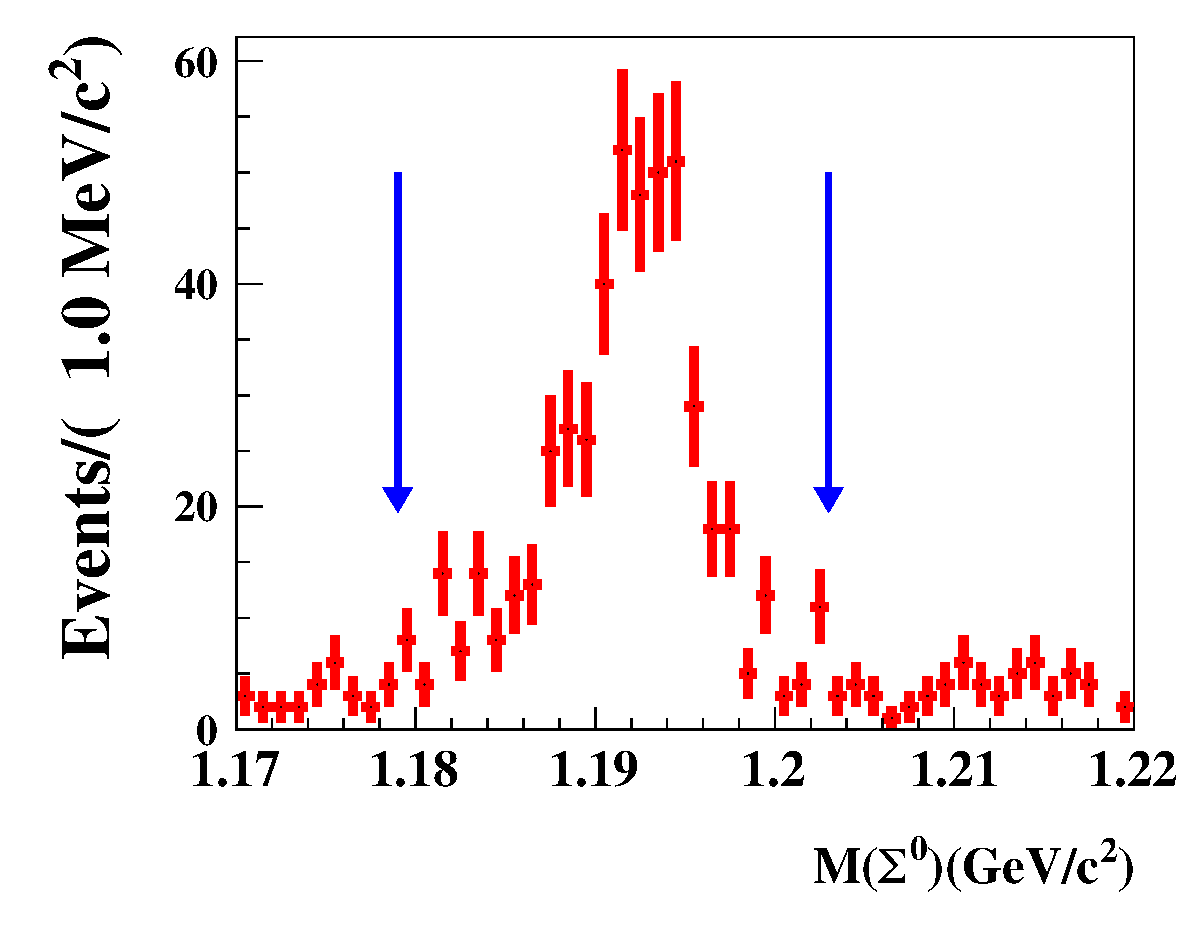
\includegraphics[width=0.45\textwidth]{chap2_m_Sgm0}
\label{fig:Sgm0mass}
}
\subfigure[数据中$\Sigmap$ 不变质量分布。]
{
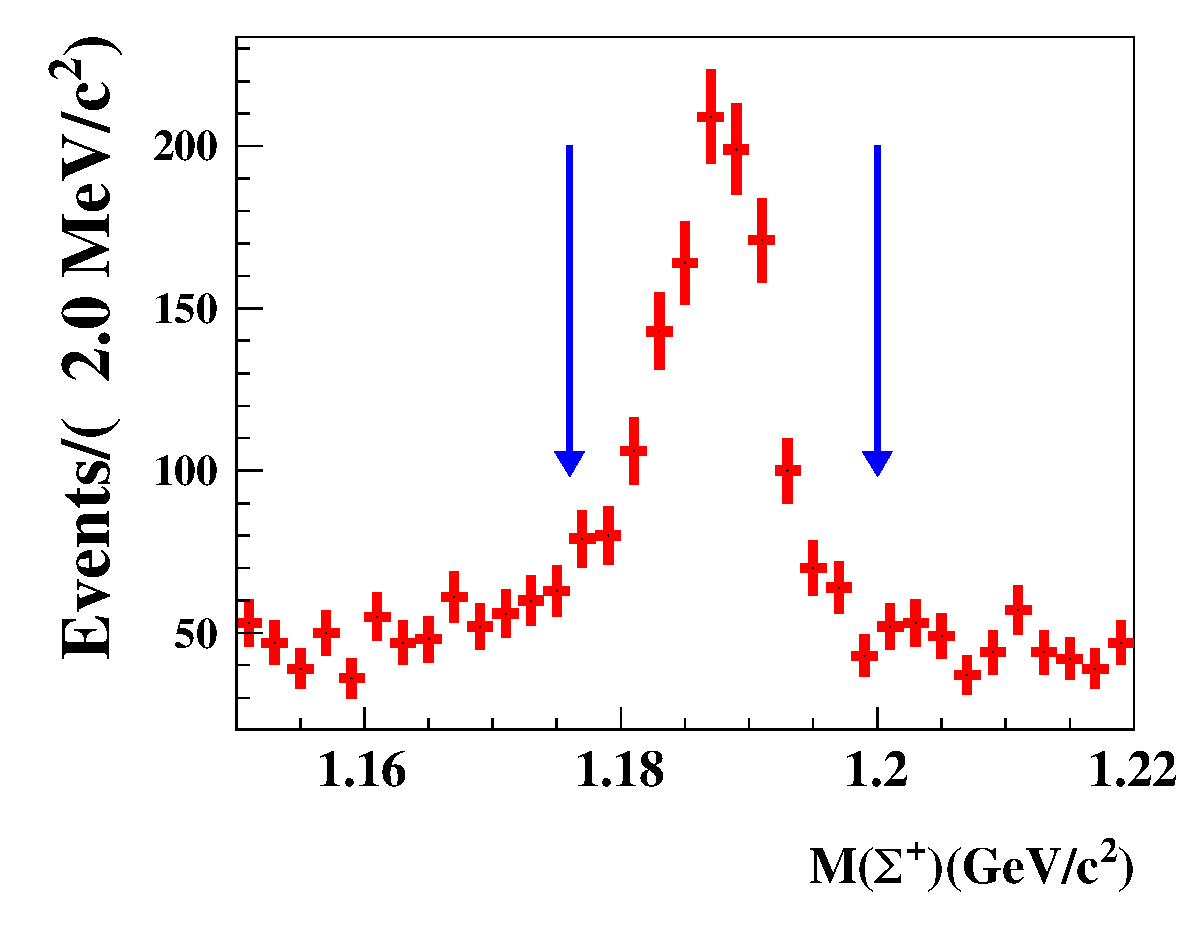
\includegraphics[width=0.45\textwidth]{chap2_m_Sgmp}
\label{fig:Sgmpmass}
}
\caption{数据中各中间共振态的不变质量谱的分布。}
\label{fig:intermediate}
\end{figure*}
%%%%%%%%%%%%%%%%%%%%%%%%%%%%%


\subsection{带电径迹的判选}

带电径迹由~MDC 重建,须成功地经过~Kalman 拟合。
Kalman 拟合使用~Kalman 滤波方法,考虑磁场的不均匀性和径迹的多次散射,对径迹进行拟合,以提高径迹动量的测量精度。

好的带电径迹还应满足以下要求:

\begin{itemize}
  \item 径迹和$e^{+}e^{-}$ 对撞点(IP)最近的距离在x-y平面上满足: $|dr|<$1 cm;在z平面上满足: $|dz|<$10 cm。即要求径迹来自对撞顶点,以排除宇宙线或束流本底。
  \item $|\cos\theta|<0.93$,即在探测器接受度以内。
\end{itemize}


筛选出好的带电径迹之后,需要对其进行分类,即,判断每条径迹的粒子类型。
我们使用~BESIII 物理分析通用的PID程序包来鉴别粒子类型。
该程序包联合~$dE/dx$ 信息和~TOF 的时间信息,计算出一条径迹为 ~$e$、$\mu$、$\pi$、$K$、$p$ 这五种粒子的概率(Probability)。
通过比较这些~Probability 值,来区分不同的粒子类型:

\begin{itemize}
%\item 对于质子(~$p$ ),要求~\footnote{对于质子的PID,由于研究发现默认的$|\chi|$值小于4要求的太严,不适合质子,所以我们要求其小于4。具体请参考章节\ref{sec:tof_chi}}:prob($p$)$\geqslant$0$\&\&$prob($p$)$\geqslant$prob($K$)$\mathcal{\&\&}$prob($p$)$\geqslant$prob($\pi$)
\item 对于质子(~$p$ ),要求: prob($p$)$\geqslant$0$\&\&$prob($p$)$\geqslant$prob($K$)$\mathcal{\&\&}$prob($p$)$\geqslant$prob($\pi$)
\item 对于~$K$ 介子,要求:prob($K$)$\geqslant$0$\mathcal{\&\&}$prob($K$)$\geqslant$prob($\pi$)
\item 对于~$\pi$ 介子,要求:prob($\pi$)$\geqslant$0$\mathcal{\&\&}$prob($\pi$)$\geqslant$prob($K$)
\end{itemize}

\subsection{中性径迹的判选}
中性径迹,即光子,由它在~EMC中的簇射中来重建,并且需要把带电径迹在~EMC 中的击中排除在外。 好光子需要满足以下条件:
\begin{itemize}
  \item 桶部光子 ($|\cos\theta|<$\rm 0.8): $E>$25 MeV
  \item 端盖光子 (0.84$<|\cos\theta|<$\rm 0.92): $E>$50 MeV
  \item 要求EMC shower的时间:$0\leq T\leq 14(\times$50 ns),$T$ 是光子的~shower在~EMC 中的~TDC时间与事例起始时间的差。
\end{itemize}

对于有带电径迹的事例,往往要求~EMC~簇射与所有带电径迹的夹角都大于~$10\,^{\circ}$或者大于~$20\,^{\circ}$。
这个夹角是光子在~EMC 中的簇射团的中心晶体的位置与带电径迹外推到~EMC 中的径迹的夹角。
这个要求,可以排除一些由于带电粒子的簇射劈裂和韧致辐射或带电径迹在~EMC 中的击中未能与该径迹匹配等原因产生的假光子。
不过由于我们的运动学约束的已经比较好了,在该分析中并没有对此有要求。

\subsection{$\pi^{0}$的重建}
中性粒子$\pi^{0}$是通过一对好光子来重建的。
我们使用~BESIII 官方的软件包~Pi0EtaToGGRecAlg 来重建。用于重建~$\pi^{0}$ 的两个光子,须满足上面列出的好光子的判选条件。
由于$\pi^{0}$的宽度较窄,相对于探测器分辨,其不变质量可以认为是一个常数。
我们可以利用这个信息将末态两个光子的四动量进行约束~\cite{Kmfit}。
这是一个1维的质量约束,我们称为1C(1-Constrain)。我们通过要求运动学拟合的$\chi^{2}$小于一定值来排除本底。
并且在运动学拟合后,更新两个光子的四动量,这个更新后的四动量被认为更准确,它将用于之后的计算和分析。
对于初步选出的$\pi^{0}$的候选者,我们要求:
\begin{itemize}
\item 不变质量窗: 0.115 $\rm GeV/c^{2}<M_{\gamma\gamma}<$0.150 $\rm GeV/c^{2}$.
\item 1C运动学约束的$\chi^{2}<$200.
\end{itemize}

\subsection{$\Ks$ ($\Lambda$) 的重建}
$K_{S}^{0}$($\Lambda$)是通过它的衰变末态$\pi^{+}\pi^{-}$($p\pi^{-}$)来重建的。因为$\Ks$($\Lambda$)寿命较长,在衰变之前它可以飞行一段距离,它的衰变顶点可以距对撞顶点有一定距离。
这样在挑选它的子粒子时,和好径迹的挑选条件不同:要求径迹在探测器的接受度以内($|cos\theta|<$\rm0.93),且起始点距束流位置在z方向的距离在20 cm以内($|\delta z|<$20 cm)。
一般在选择$K_{S}^{0}$($\Lambda$)时是不对末态这两条径迹做粒子类型的鉴别的,但是研究发现如果对$p$做个PID的要求,会显著改善信噪比,同时效率也基本没有变化。
BESIII实验上对于此类有衰变顶点的粒子往往运用顶点拟合和次级顶点拟合的方法来区别$K_{S}^{0}$($\Lambda$)信号和本底~\cite{vfit}。
所谓顶点拟合就是要求两条带电径迹来自同一个顶点,次级顶点拟合就是判断$\Ks$($\Lambda$)衰变顶点的位置,要求$\Ks$($\Lambda$)的衰变顶点距对撞顶点有一定距离。
总的来说,我们对$\Ks$($\Lambda$)的挑选条件是:
\begin{itemize}
  \item $\pip$ 和$\pim$ ($p$ 和$\pim$) 满足 $|\delta z|<20\,\unit{cm}$, $|cos\theta|<0.93$
  \item 对$\pi$没有PID的要求。
  \item 质子 PID 要求:  prob($p$)$\geqslant$0$\&\&$prob($p$)$\geqslant$prob($K$)$\mathcal{\&\&}$prob($p$)$\geqslant$prob($\pi$)
  \item $\Ks$($\Lambda$)不变质量要求: $0.487\rm \ GeV/c^{2}<M_{\pip\pim}<\rm 0.511\rm \ GeV/c^{2}$~($1.111\rm \ GeV/c^{2}<M_{p\pim}<\rm 1.121\rm \ GeV/c^{2}$)
  \item 顶点拟合: $\chi^{2}<$100
  \item 次级顶点拟合找到的$K_{S}^{0}$($\Lambda$)的衰变顶点和对撞顶点有明显区分:$L/\sigma_{L}>$2, 其中$L$指$K_{S}^{0}$($\Lambda$)的衰变长度(飞行距离),$\sigma_{L}$指$L$的误差。它们是通过次级顶点拟合取得的。
\end{itemize}

\subsection{$\Sigmazero$和$\Sigmap$的重建}
$\Sigmazero$是通过它的衰变末态$\Lambda\gm$来重建的。
$\Sigmap$通过$p \pizero$来重建。
其中子粒子$\Lambda$、$\pip$、$\pim$、$\pizero$和$\gm$的选择条件和前面所述一致。
$\Sigmazero$ 的不变质量要求为$1.179<M_{\Lambda\gm}<1.203\gevcc$。
$\Sigmap$ 的不变质量要求为$1.176<M_{p \pizero}<1.20\gevcc$。

